\documentclass{beamer}
\usepackage{beamerthemesplit}
\usepackage{wrapfig}
\usetheme{SPbGU}
\usepackage{pdfpages}
\usepackage{amsmath}
\usepackage{cmap} 
\usepackage[T2A]{fontenc} 
\usepackage[utf8]{inputenc}
\usepackage[english,russian]{babel}
\usepackage{indentfirst}
\usepackage{amsmath}
\usepackage{tikz}
\usepackage{multirow}
\usepackage[noend]{algpseudocode}
\usepackage{algorithm}
\usepackage{algorithmicx}
\usetikzlibrary{shapes,arrows}
%usepackage{fancyvrb}
%\usepackage{minted}
%\usepackage{verbments}


\newtheorem{rutheorem}{Теорема}
\newtheorem{ruproof}{Доказательство}
\newtheorem{rudefinition}{Определение}
\newtheorem{rulemma}{Лемма}
\beamertemplatenavigationsymbolsempty

\title[]{Parsing techniques for graph analysis}
%\subtitle[YaccConstructor]{Parsing techniques for graph analysis}
% То, что в квадратных скобках, отображается в левом нижнем углу. 
\institute[SPbU]{
JetBrains Research, Programming Languages and Tools Lab  \\
Saint Petersburg University
}

% То, что в квадратных скобках, отображается в левом нижнем углу.
\author[Ekaterina Verbitskaia]{Ekaterina Verbitskaia}

\date{Oktober 22, 2017}

\definecolor{orange}{RGB}{179,36,31}

\begin{document}
{
\begin{frame}[fragile]
  \begin{tabular}{p{2.5cm} p{5.5cm} p{2cm}}
   \begin{center}
      
\includegraphics[height=1.5cm]{pictures/JBLogo3.pdf}
    \end{center}
    &
    \begin{center}
      
\includegraphics[height=1.5cm]{pictures/SPbGU_Logo.png}
    \end{center}
    &
    \begin{center}
      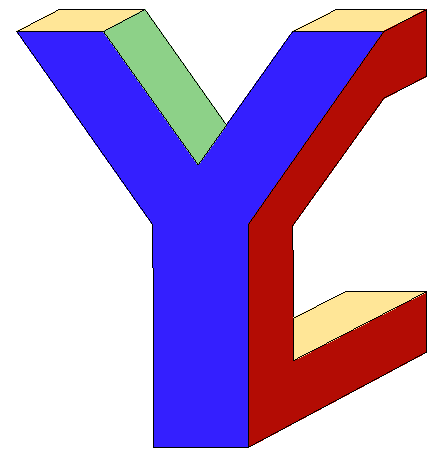
\includegraphics[height=1.5cm]{pictures/YC_logo.pdf}
    \end{center} 
  \end{tabular}
  \titlepage
\end{frame}
}

\begin{frame}[fragile]
  \transwipe[direction=90]
  \frametitle{Paths with constraints}
  \begin{itemize}
    \item Graph DB querying
    \item Static cide analysis
    \item ...
  \end{itemize}
\end{frame}


\begin{frame}[fragile]
  \transwipe[direction=90]
  \frametitle{Context-free constarints}
  \begin{itemize}
    \item $\mathbb{G} = (\Sigma, N, P)$ --- context-free grammar
    \item $G = (V,E,L)$ --- directed graph, $E \subseteq V\times L \times V$, $L\subseteq \Sigma$
    \item $p=(v_0,l_0,v_1),\cdots,(v_{n-1},l_{n-1},v_n)$ --- path in $G$
    \item $\omega(p) = \omega((v_0,l_0,v_1),\cdots,(v_{n-1},l_{n-1},v_n)) = l_0 l_1 \cdots l_{n-1}$
    \item $R =\{ p | \exists N_i \in N (\omega(p) \in L(\mathbb{G},N_i))\}$
  \end{itemize}
\end{frame}

\begin{frame}
  \transwipe[direction=90]
  \frametitle{Bar-Hillel theorem!}
  \begin{itemize}
    \item Bar-Hillel theorem!
    \item Parsing algorithms are constructive proof of BH theorem for one simple case...
  \end{itemize}
\end{frame}

\begin{frame}
  \transwipe[direction=90]
  \frametitle{OPen Problems etc}
  \begin{itemize}
    \item 
  \end{itemize}
\end{frame}

\begin{frame}
  \transwipe[direction=90]
  \frametitle{GLL-based}
  \begin{itemize}
    \item 
  \end{itemize}
\end{frame}

\begin{frame}
  \transwipe[direction=90]
  \frametitle{Combinators}
  \begin{itemize}
    \item 
  \end{itemize}
\end{frame}

\begin{frame}
  \transwipe[direction=90]
  \frametitle{Matrix}
  \begin{itemize}
    \item 
  \end{itemize}
\end{frame}

\begin{frame}[fragile]
\transwipe[direction=90]
\frametitle{Future work}
\begin{itemize}
  \item Other grammars and languages intersection
  \item Mechaniation on Coq
  \item Applications 
\end{itemize}
\end{frame}
            
\begin{frame}
\transwipe[direction=90]
\frametitle{Information}
\begin{itemize}
  \item \url{semen.grigorev@jetbrains.com}
  \item \url{kajigor@gmail.com}
  \item YaccConstructor: \url{https://github.com/YaccConstructor}
\end{itemize}
\end{frame}
\end{document}
